\documentclass[conference]{IEEEtran}
\usepackage[utf8]{inputenc}
\usepackage{amsmath}
\usepackage{booktabs}
\usepackage{verbatim}
\usepackage{graphicx}

\title{Labwork 2: Linear Regression}
\author{\IEEEauthorblockN{Nguyen Phong Chau}
\IEEEauthorblockA{Student ID 2540008\\
University of Science and Technology of Hanoi}
}

\begin{document}

\onecolumn

\maketitle

\begin{abstract}
This lab work reports a linear regression experiment using gradient descent on a dataset. The study evaluates the convergence behaviour and final model performance.
\end{abstract}

\section{Introduction}

The dataset consists of pairs of input-output values, and the goal is to fit a linear model of the form $y = w_0 + w_1 x$ to the data. The mean squared error (MSE) is used as the loss function, defined as:
\[\text{MSE}(w) = \frac{1}{n} \sum_{i=1}^{n} (w_0 + w_1 x_i - y_i)^2\]
The gradients of the loss function with respect to the weights are computed as follows:
\[\frac{\partial \text{MSE}}{\partial w_0} = \frac{2}{n} \sum_{i=1}^{n} (w_0 + w_1 x_i - y_i)\]
\[\frac{\partial \text{MSE}}{\partial w_1} = \frac{2}{n} \sum_{i=1}^{n} x_i (w_0 + w_1 x_i - y_i)\]


\section{Implementation}


The experiment uses initial value $w=(5.0, 2.0)$, learning rate $\eta=2.5 \times 10^{-4}$, and convergence threshold $\epsilon=10^{-6}$. The training loop iteratively updates the weights until the change in loss is less than $\epsilon$.

The training algorithm is implemented as follows:

\begin{verbatim}
def training_loop(weight, lr, epsilon):
    time = 0
    y_pred = [predict(x_i, weight) for x_i in x_train]
    current_loss = loss(y_pred, y_train, weight)
    delta = 10

    while delta > epsilon:
        weight = grad_descent(x_train, y_train, weight, lr)
        y_pred = [predict(x_i, weight) for x_i in x_train]
        delta = abs(current_loss - loss(y_pred, y_train, weight))

        current_loss = loss(y_pred, y_train, weight)
        time += 1
        # print(time, weight, current_loss, delta)
    return time, weight, current_loss
\end{verbatim}

\section{Results}

The model converged after 96344 iterations, yielding a final weight of approximately $(47.98771292513566, 1.262196718006951)$ and a final MSE loss of $5636.464636021761$. 

The final regression line compare to the original data points is shown in Figure~\ref{fig:convergence}.

\begin{figure}[ht]
    \centering
    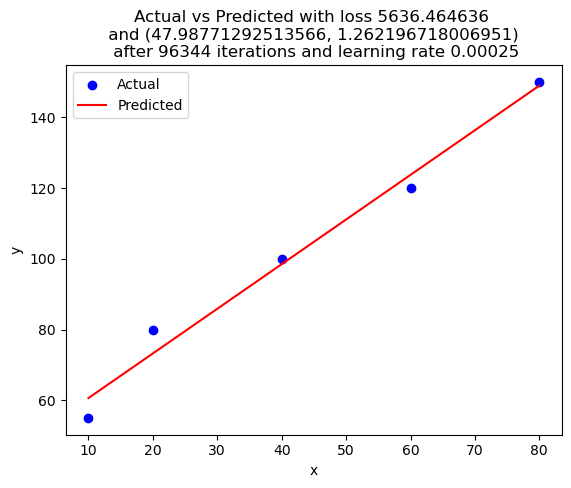
\includegraphics[width=1\textwidth]{output.png}
    \caption{Convergence of weights and loss over iterations}
    \label{fig:convergence}
\end{figure}

\section{Discussion}

Experimenting different learning rates revealed that $\eta=4 \times 10^{-4}$ provided the fastest convergence time. The training converges faster with larger learning rates, but the current algorithm caught an overflow error from $\eta>=5 \times 10^{-4}$.

The relation between learning rate and convergence time is shown in the Figure~\ref{fig:lr_convergence}.

\begin{figure}[ht]
    \centering
    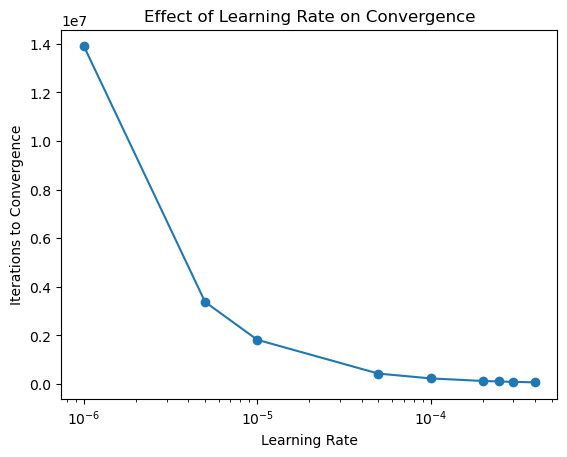
\includegraphics[width=1\textwidth]{lr_convergence.png}
    \caption{Convergence time for different learning rates}
    \label{fig:lr_convergence}
\end{figure}


\end{document}